
\documentclass[
	% -- opções da classe memoir --
	article,			% indica que é um artigo acadêmico
	11pt,				% tamanho da fonte
	oneside,			% para impressão apenas no verso. Oposto a twoside
	a4paper,			% tamanho do papel. 
	% -- opções da classe abntex2 --
	%chapter=TITLE,		% títulos de capítulos convertidos em letras maiúsculas
	%section=TITLE,		% títulos de seções convertidos em letras maiúsculas
	%subsection=TITLE,	% títulos de subseções convertidos em letras maiúsculas
	%subsubsection=TITLE % títulos de subsubseções convertidos em letras maiúsculas
	% -- opções do pacote babel --
	english,			% idioma adicional para hifenização
	brazil,				% o último idioma é o principal do documento
	]{abntex2}


% ---
% PACOTES
% ---

% ---
% Pacotes fundamentais 
% ---
\usepackage{cmap}				% Mapear caracteres especiais no PDF
\usepackage{lmodern}			% Usa a fonte Latin Modern
\usepackage[T1]{fontenc}		% Selecao de codigos de fonte.
\usepackage[utf8]{inputenc}		% Codificacao do documento (conversão automática dos acentos)
\usepackage{indentfirst}		% Indenta o primeiro parágrafo de cada seção.
\usepackage{nomencl} 			% Lista de simbolos
\usepackage{color}				% Controle das cores
\usepackage{graphicx}			% Inclusão de gráficos
\usepackage{csvsimple}
% ---
		
% ---
% Pacotes adicionais, usados apenas no âmbito do Modelo Canônico do abnteX2
% ---
\usepackage{lipsum}				% para geração de dummy text
% ---
		
% ---
% Pacotes de citações
% ---
\usepackage[brazilian,hyperpageref]{backref}	 % Paginas com as citações na bibl
\usepackage[alf]{abntex2cite}	% Citações padrão ABNT
% ---

% ---
% Configurações do pacote backref
% Usado sem a opção hyperpageref de backref
\renewcommand{\backrefpagesname}{Citado na(s) página(s):~}
% Texto padrão antes do número das páginas
\renewcommand{\backref}{}
% Define os textos da citação
\renewcommand*{\backrefalt}[4]{
	\ifcase #1 %
		Nenhuma citação no texto.%
	\or
		Citado na página #2.%
	\else
		Citado #1 vezes nas páginas #2.%
	\fi}%
% ---

% ---
% Informações de dados para CAPA e FOLHA DE ROSTO
% ---
\titulo{Relatório de atividades: Uso do classificador 1-NN, KNN e DMC na base
de dados da flor de íris} 
\autor{David Clifte\thanks{cliftedavid@gmail.com}}
\local{Brasil}
\data{2015, v-1.0}
% ---

% ---
% Configurações de aparência do PDF final

% alterando o aspecto da cor azul
\definecolor{blue}{RGB}{41,5,195}

% informações do PDF
\makeatletter
\hypersetup{
     	%pagebackref=true,
		pdftitle={\@title}, 
		pdfauthor={\@author},
    	pdfsubject={Modelo de artigo científico com abnTeX2},
	    pdfcreator={LaTeX with abnTeX2},
		pdfkeywords={abnt}{latex}{abntex}{abntex2}{atigo científico}, 
		colorlinks=true,       		% false: boxed links; true: colored links
    	linkcolor=blue,          	% color of internal links
    	citecolor=blue,        		% color of links to bibliography
    	filecolor=magenta,      		% color of file links
		urlcolor=blue,
		bookmarksdepth=4
}
\makeatother
% --- 

% ---
% compila o indice
% ---
\makeindex
% ---

% ---
% Altera as margens padrões
% ---
\setlrmarginsandblock{4cm}{4cm}{*}
\setulmarginsandblock{4cm}{4cm}{*}
\checkandfixthelayout
% ---

% --- 
% Espaçamentos entre linhas e parágrafos 
% --- 

% O tamanho do parágrafo é dado por:
\setlength{\parindent}{1.3cm}

% Controle do espaçamento entre um parágrafo e outro:
\setlength{\parskip}{0.2cm}  % tente também \onelineskip

% Espaçamento simples
\SingleSpacing

% ----
% Início do documento
% ----
\begin{document}

% Retira espaço extra obsoleto entre as frases.
\frenchspacing 

% ----------------------------------------------------------
% ELEMENTOS PRÉ-TEXTUAIS
% ----------------------------------------------------------

%---
%
% Se desejar escrever o artigo em duas colunas, descomente a linha abaixo
% e a linha com o texto ``FIM DE ARTIGO EM DUAS COLUNAS''.
% \twocolumn[    		% INICIO DE ARTIGO EM DUAS COLUNAS
%
%---
% página de titulo
\maketitle

% resumo em português
\begin{resumoumacoluna}
 Este trabalho apresentam os resultados obtidos ao aplicar os classificadores
 1-nn, KNN e DMC ao banco de dados da íris. A implementação foi feita no
 Matlab\texttrademark 
 
 
 \vspace{\onelineskip}
 
 \noindent
 \textbf{Palavras-chaves}: latex. abntex. editoração de texto.
\end{resumoumacoluna}

% ]  				% FIM DE ARTIGO EM DUAS COLUNAS
% ---

% ----------------------------------------------------------
% ELEMENTOS TEXTUAIS
% ----------------------------------------------------------
\textual

% ----------------------------------------------------------
% Introdução
% ----------------------------------------------------------
\section*{Introdução}


% ----------------------------------------------------------
% Seção de explicações
% ----------------------------------------------------------
\section{Preparação da base}
\subsection{Base de dados da flor de íris}
A base de dados da flor de íris criado por Fisher \cite{AHG2137}. Nessa base de
dados as informações obtidas das flores foram o comprimento e a largura das
pétalas e sépalas de 3 tipos de flor de íris, virgínica, versicolor e setosa.
Cada tipo de flor possue 50 instancias.

\subsection{Normalização e codificação}
\label{ss:normCodf} 
Após o carregamento da base foi realizado apenas a normalização dos dados e a
codificação dos rótulos. A normalização foi realizada separadamente para cada
atributo. Foi identificado o máximo e o mínimo do atributo $p$ e todos os
valores foram normalizados na faixa [0,1].

A codificação do rótulo foi feita no modelo 1-de-k(1-of-K ou one-hot encoding),
nesse modelo o rótulo é codificado em um vetor onde cada posição do
vetor representa uma classe. Nesse modelo para uma quantidade $m$ de classes
temos um vetor com $m$ posições e a classe $k$ é representada por um vetor
onde todas as outras posições diferentes de $k$ possuem o valor zero e a
posição $k$ possui o valor 1. Dessa forma as três classes possíveis da íris
foram codificadas em um vetor de 3 posições, onde a posição 1, 2 e 3
representam a classe setosa, versicolor e virgínica respectivamente.


%Gráfico em barra
\subsection{Análise das características}

Na figura \ref{fig:charMatrix} é apresentada a matriz de características. 
Essa matriz consiste de gráficos formados pelos pares de características
combinadas.

Na diagonal principal é apresentado o histograma do atributo.
Devido a natureza continua dos atributos do problema, pois o
comprimento e largura da sépala e pétala podem assumir qualquer valor real O
histograma foi obtido após a realização da quantização dos atributos.
Cada atributo foi quantizado em 15 possíveis valores com faixas de mesma largura. A
largura da faixa foi obtida da seguinte forma $(max_p - min_p)/15$, onde max e
min são os valores máximos e mínimos do atributo $p$.

\begin{figure}[!htb] \centering
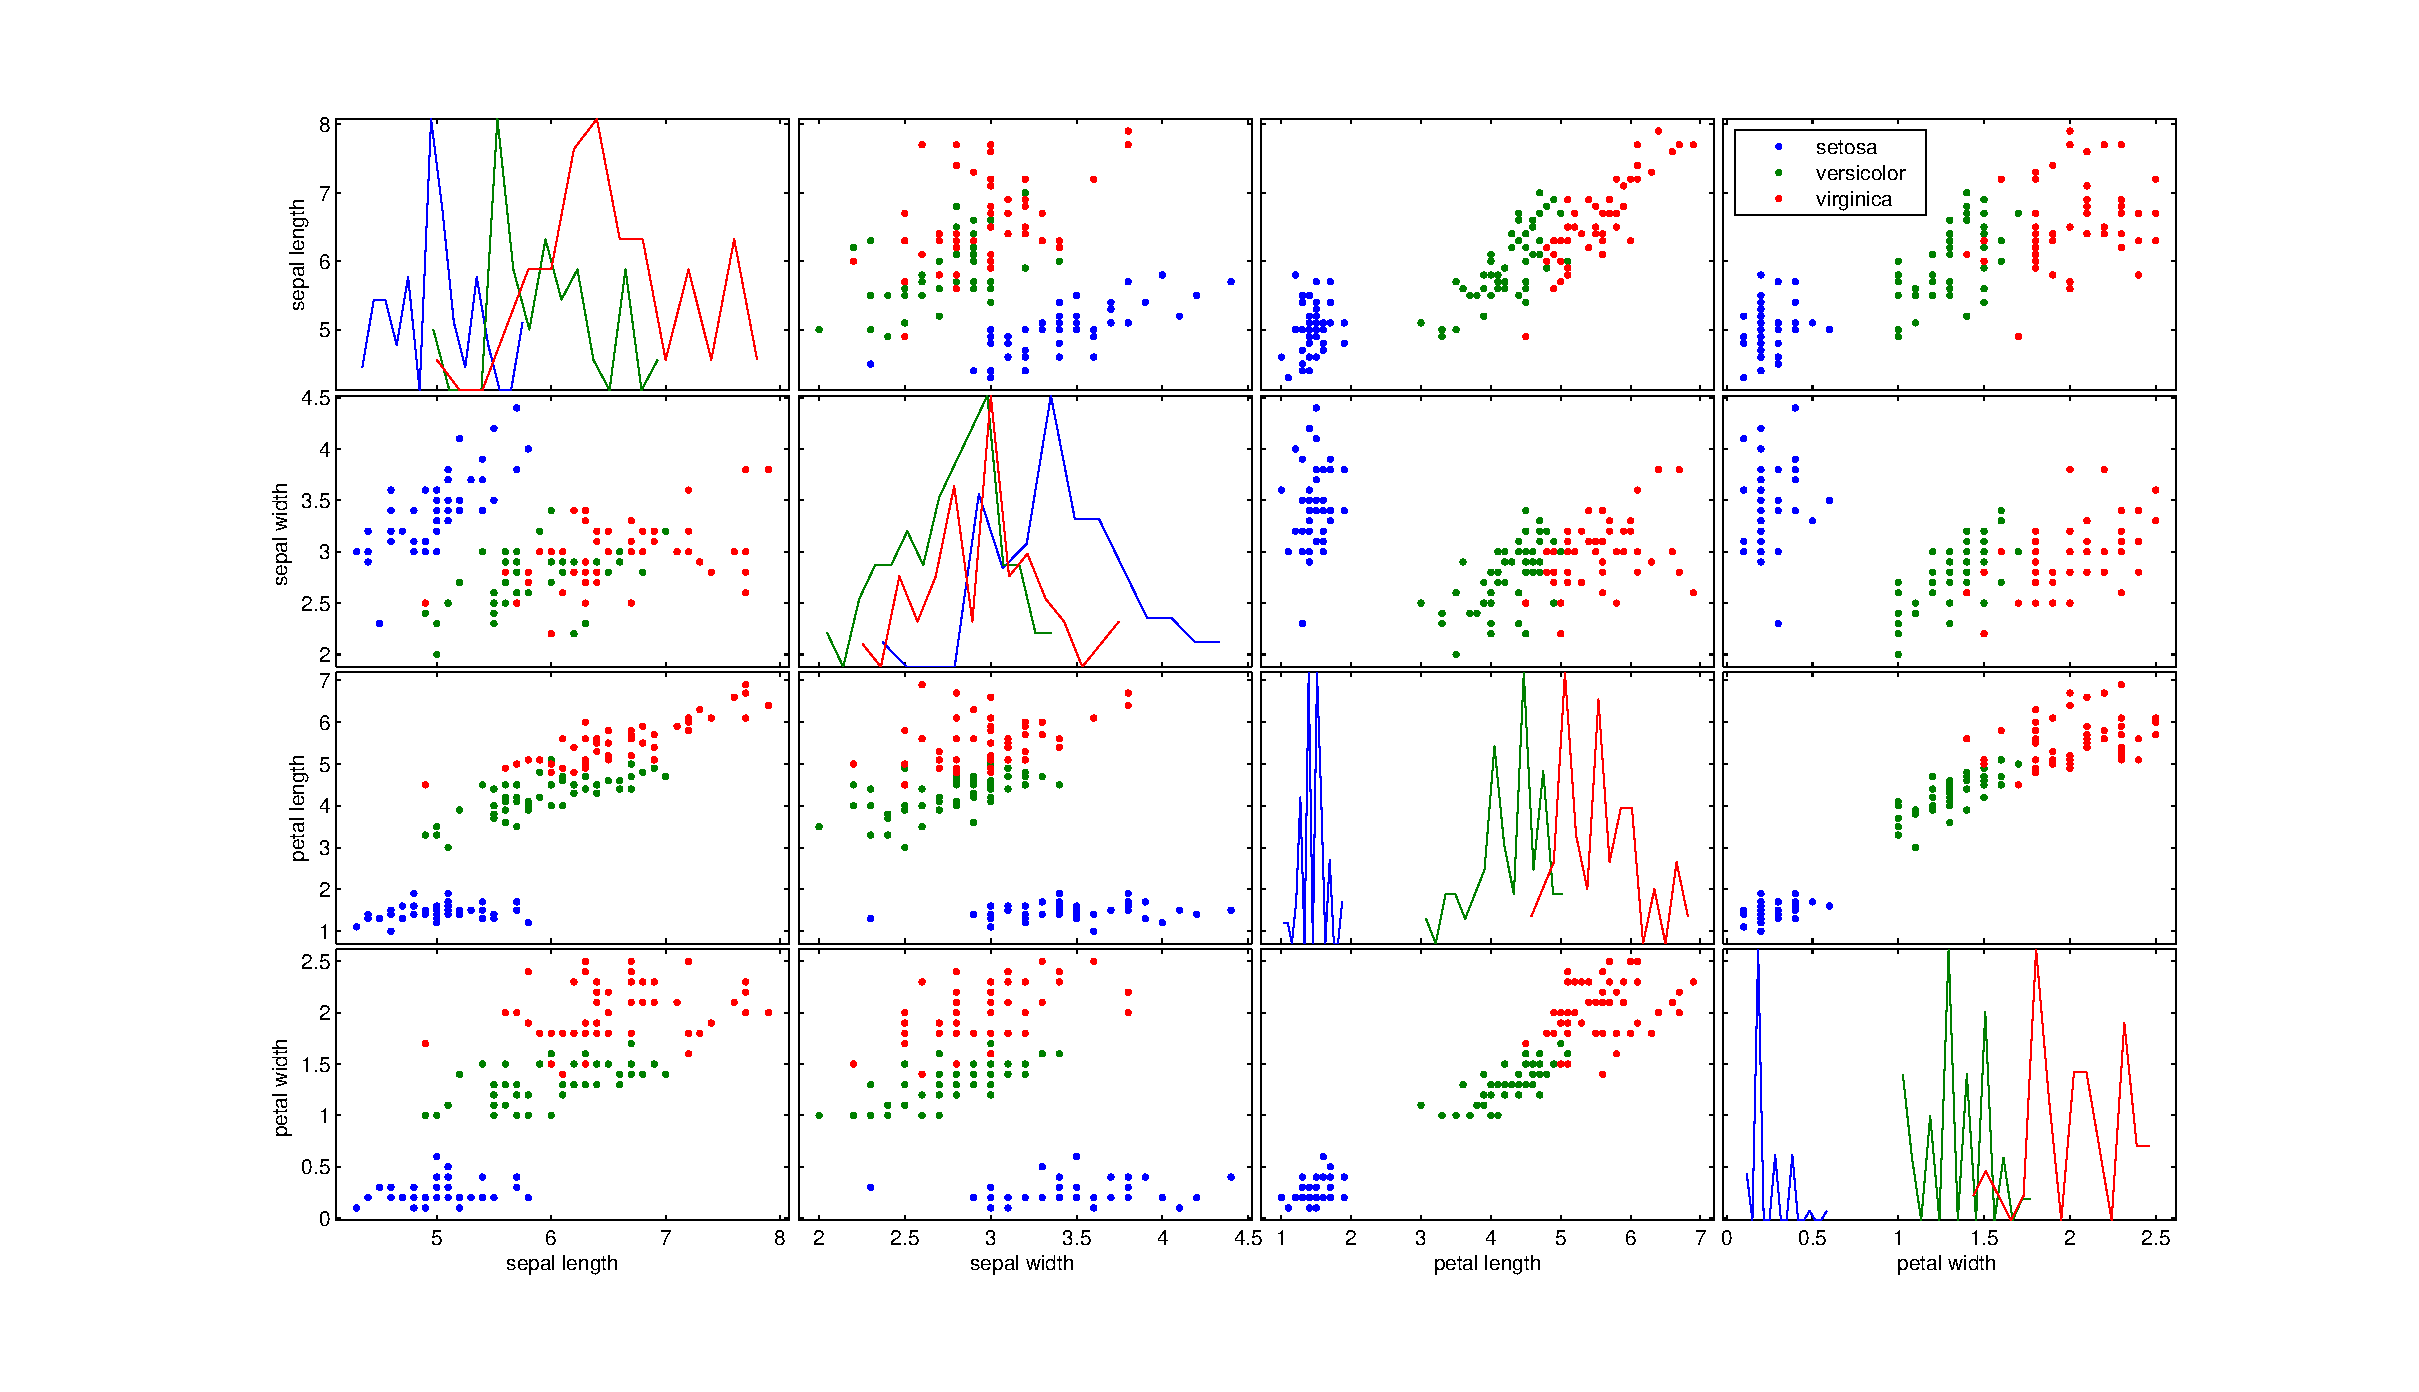
\includegraphics[width=\textwidth]{figuras/analiseIris_hist_scatterMatrix.eps}
\caption{Matriz de características.}
\label{fig:charMatrix}
\end{figure}

 Podemos perceber que a classe setosa pode facilmente ser separada das outras
 utilizando a largura ou o comprimento da pétala como variável. Nos histogramas
 localizados na parte inferior isso pode ser verificado, pétalas com
 comprimentos menores que 0,25 ou sépalas com largura menor que 0,3 de
 comprimento são claramente da classe setosa.
 Já para as duas outras características essa separação não é tão simples,
 perceba a sobreposição dos histogramas em todos os atributos bem como a mistura
 das classes nos gráficos de dispersão.
%  
% \subsubsection{Análise PCA}
% PCA is a standard technique for visualizing high dimensional data and for data
% pre-processing. PCA reduces the dimensionality (the number of variables) of a
% data set by maintaining as much variance as possible.
% 
% The first component, PC 1, represents the direction of the highest variance
% of the data. The direction of the second component, PC 2, represents the highest
% of the remaining variance orthogonal to the first component.
% 
%  Low variance can often be assumed to represent undesired background noise. The
% dimensionality of the data can therefore be reduced, without loss of relevant information
% 



\section{1-NN e KNN}

\subsection{Introdução}
O KNN é uma técnica que realiza a classificação de uma amotra de acordo com as k
amotras mais semelhantes existentes em sua base. Essa semelhança pode ser
quantificada atravez de uma função característica do problema ou mais comumente
atravez do calculo da distância euclidiana. O 1-NN é um caso específico do KNN
para este classificador o número de vizinhos que deve ser levado em conta é
apenas 1.

Uma importante vantagem do KNN frente ao 1-NN é a capacidade de controlar a
interferência a ruídos presentes na base de dados. Quanto maior o valor de K
mais informação será levada em consideração para a identificação da label da
amostra e considerando também que a quantidade de ruído presente próximo a
amostra é suficientemente pequena frente ao valor de K este pode ser contornado.

\subsection{Metodologia}
Para a avaliação do KNN foi realizado a normalização e a codificação das classe
no modelo 1-of-k, como dito na subsessão \ref{ss:normCodf}, além foi necessário
alguns outros passos para obtermos os resultados apresentados na sessão
seguinte.

Após a normalização e a codificação a base de dados foi dividida por um  de 1:4,
desta forma das 150 amostras presentes na base 30 delas foram escolhidas
aleatoriamente para pertencerem à base de testes e o restante, 120, pertencerem
a base de treinamento. É importante ressaltar também que pelo fato da escolha
dos dados de testes serem dados de forma aleatória não é possível garantir que a
base de treinamento ou teste possuem uma quantidade equivalente das 3 classes,
porém espera-se que existam aproximadamente 40 instancias de cada classe na base
de treinamento e 10 instancias de cada classe na base de teste.



\subsection{Resultados obtidos}
Foram feitos uma série de teste variando o valor de K bem como testes de
generalização onde foi realizado a minimização da quantidade de dados
necessários na base para uma correta classificação.

\subsection{Variação do valor de K}
Nesse teste foram realizadas 100 repetições para cada valor de K. A acurácia e o
desvio padrão são exibidos na tabela \ref{tab:acuracia}. A figura
\ref{fig:acuracia} apresenta um . 
É percebido que para o problema da íris a variação do valor de k não representa
diferença significativa para um valor de k até 30, mesmo para o valor de k igual
a 1. Para valores de K superiores a 30 podemos notar uma redução da acurácia e a
partir de 70 a média começa a dimunuir. Na faixa [60 a 110] a acurácia variou
entre 20\% e 90\% o que indica baixíssima confiabilidade no classificador. A
partir de 120 o classificar indica apenas a classe majoritária presente na base
de dados, indistintamente da amostra apresentada.

\begin{table}
	\centering
    \begin{tabular}{c|c|c}%
    \bfseries K & \bfseries Acurácia & \bfseries Desvio Padrão% specify table
    % head 
    \csvreader[no head]{matlab/iris_acuracia.csv}{}% use head of
    % csv as column names
    {\\\hline\csvcoli&\csvcolii&\csvcoliii}% specify your coloumns here
    \\\hline
    
    \end{tabular}
    \caption{Acurácia média e desvio padrão em função do valor de k.}
    \label{tab:acuracia}
\end{table}

\begin{figure}[!htb] \centering
	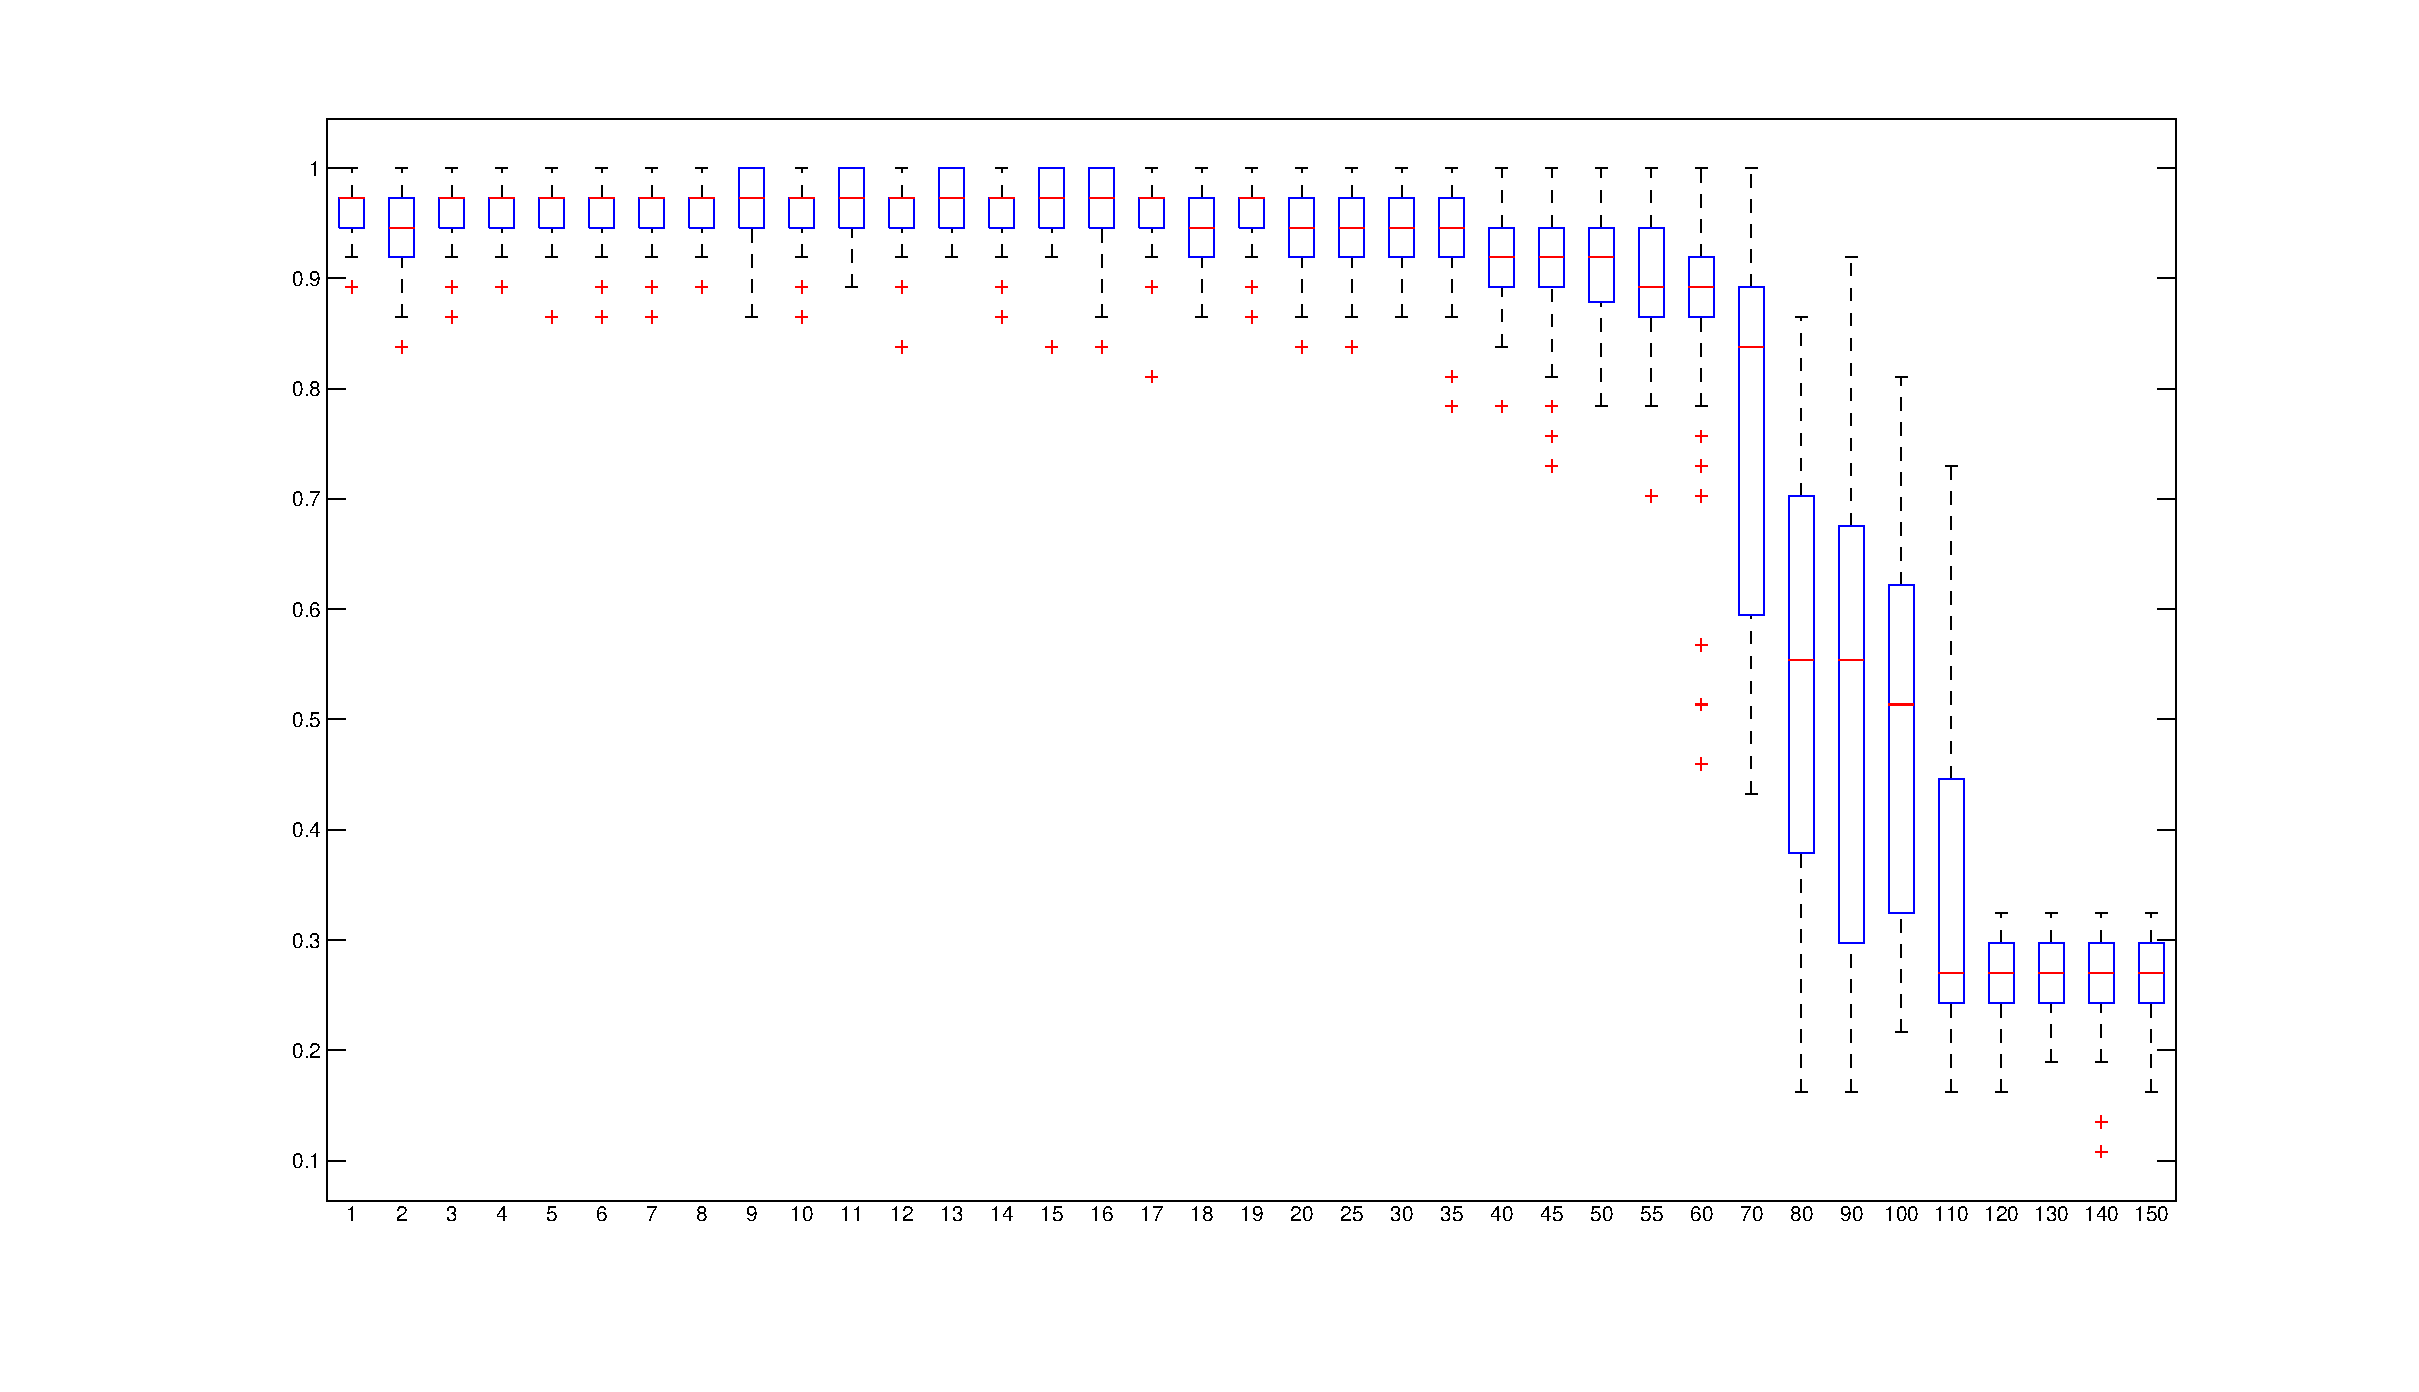
\includegraphics[width=\textwidth]{figuras/boxPlot_acuraciaVSK.eps}
	\caption{Acurácia em função do valor de k.}
	\label{fig:acuracia}
\end{figure}


\section{DMC}


\subsection{Região de decisão}

\begin{figure}
	\centering
	\begin{tabular}{cc}
	  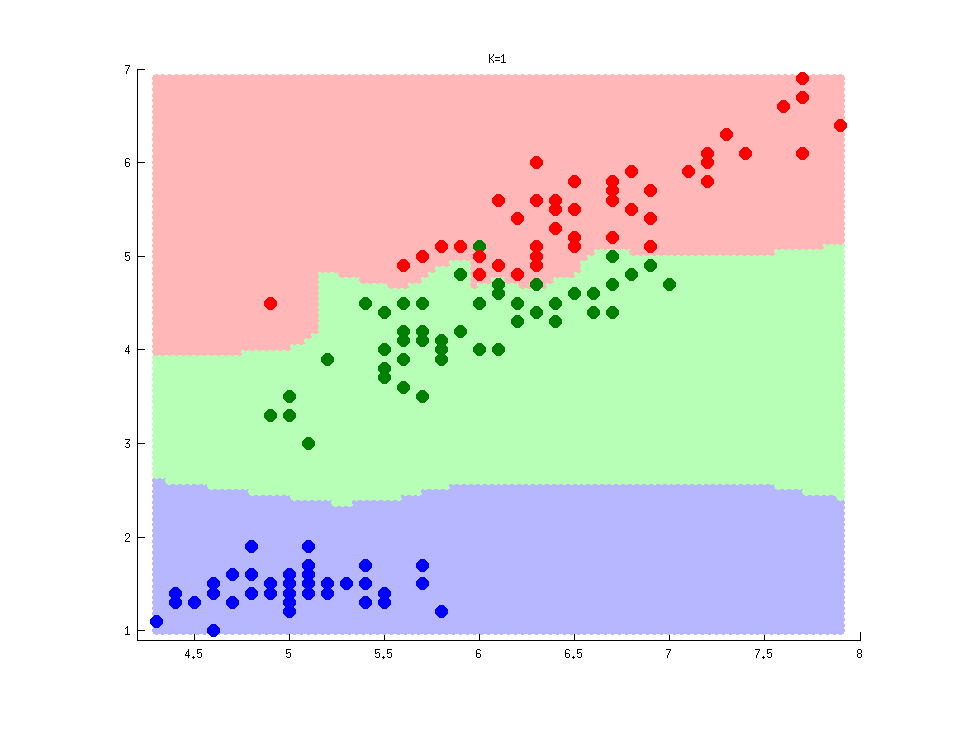
\includegraphics[width=70mm]{figuras/sepLVsPetL/decRegK1.eps} &  
	  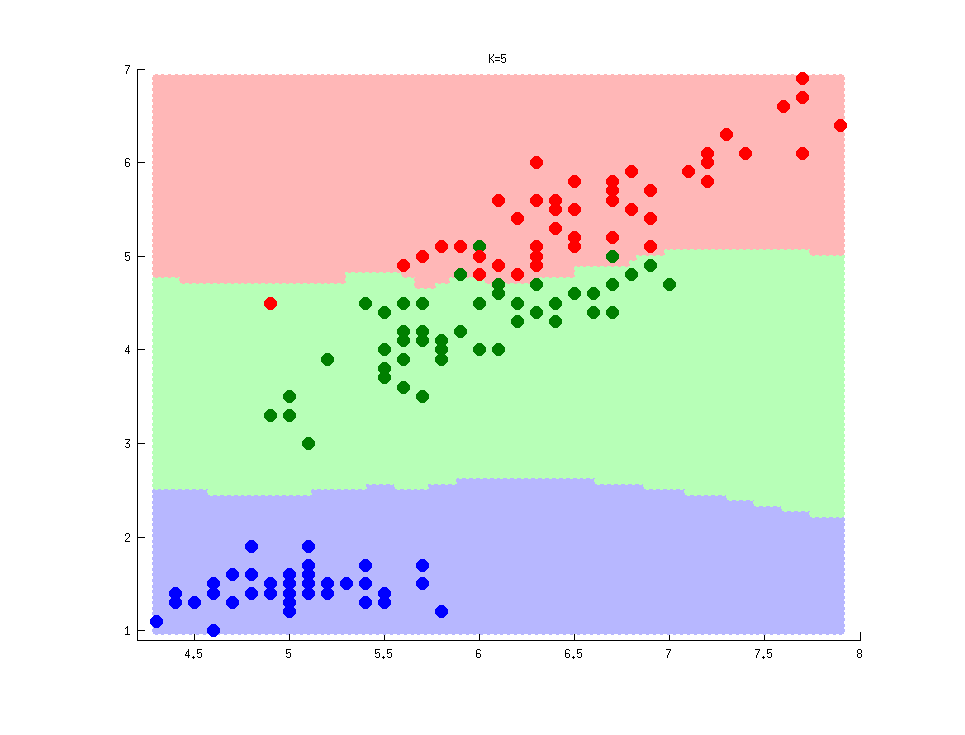
\includegraphics[width=70mm]{figuras/sepLVsPetL/decRegK5.eps}
	  \\
	(a) k=1 & (b) k=5 \\[6pt] 
	 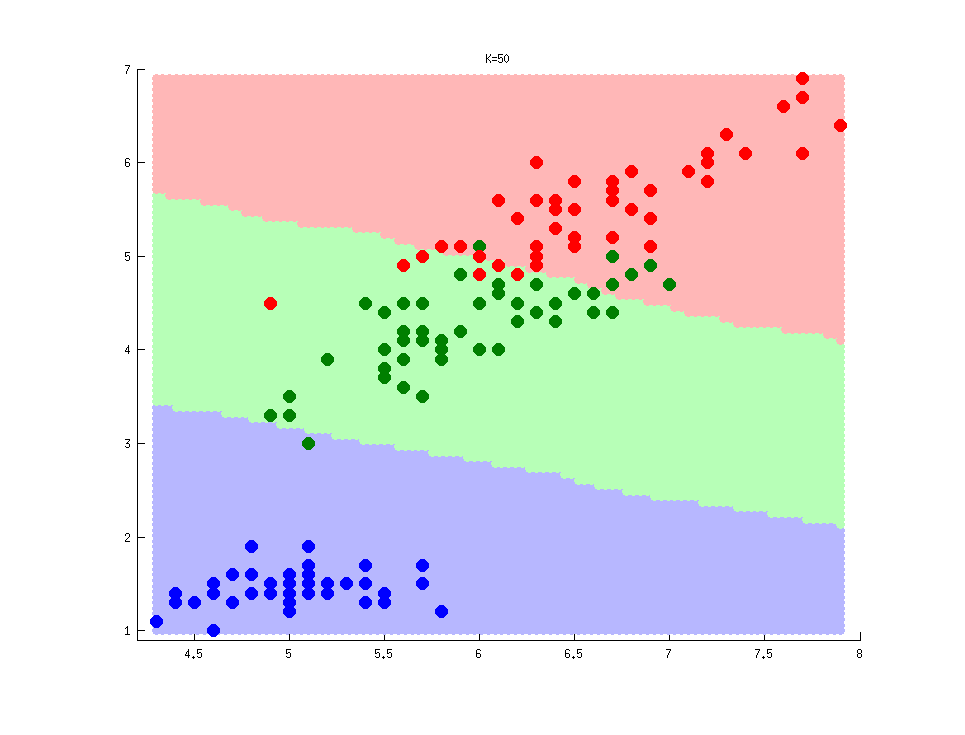
\includegraphics[width=70mm]{figuras/sepLVsPetL/decRegK50.eps} &  
	 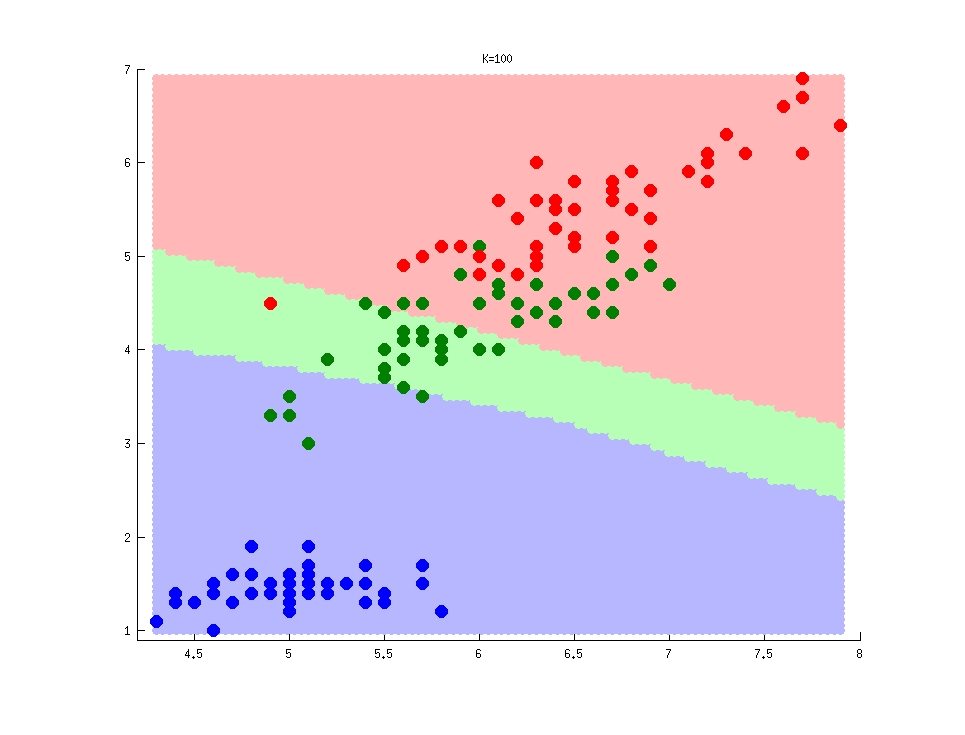
\includegraphics[width=70mm]{figuras/sepLVsPetL/decRegK100.eps} \\
	(c) k=50 & (d) k=100 \\[6pt] 

	\end{tabular}
	\label{fig:decisionRegionSepL_PetL}
	\caption{Região de decisão utilizando Largura da sépala e da pétala.}
\end{figure}

\begin{figure}
	\centering
	\begin{tabular}{cc}
	  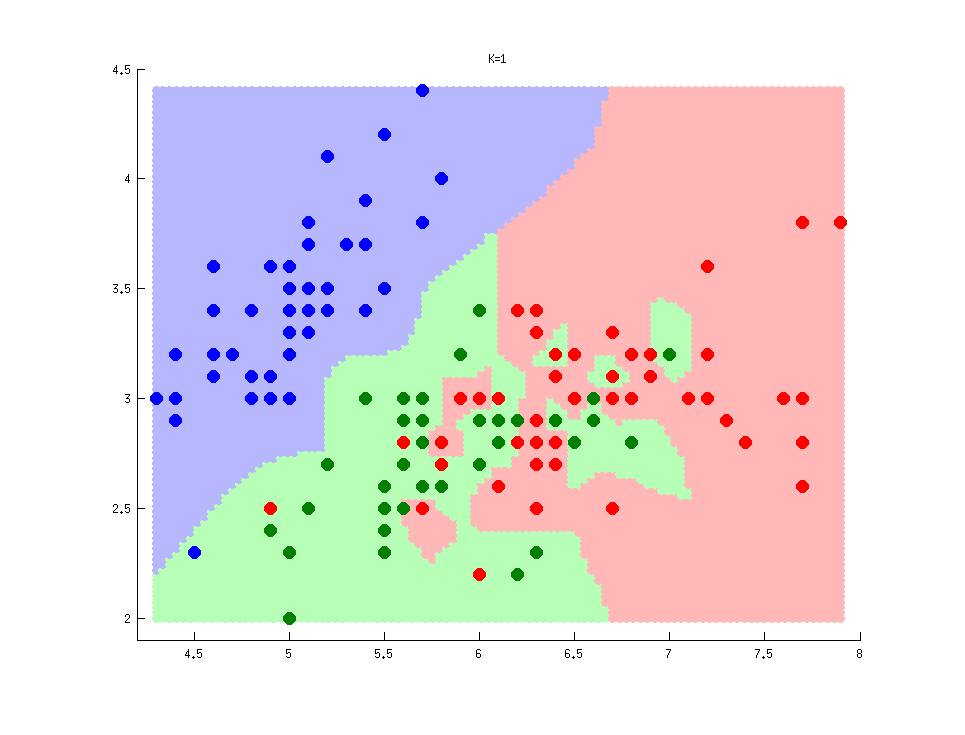
\includegraphics[width=70mm]{figuras/sepLVssepW/decRegK1.eps} &  
	  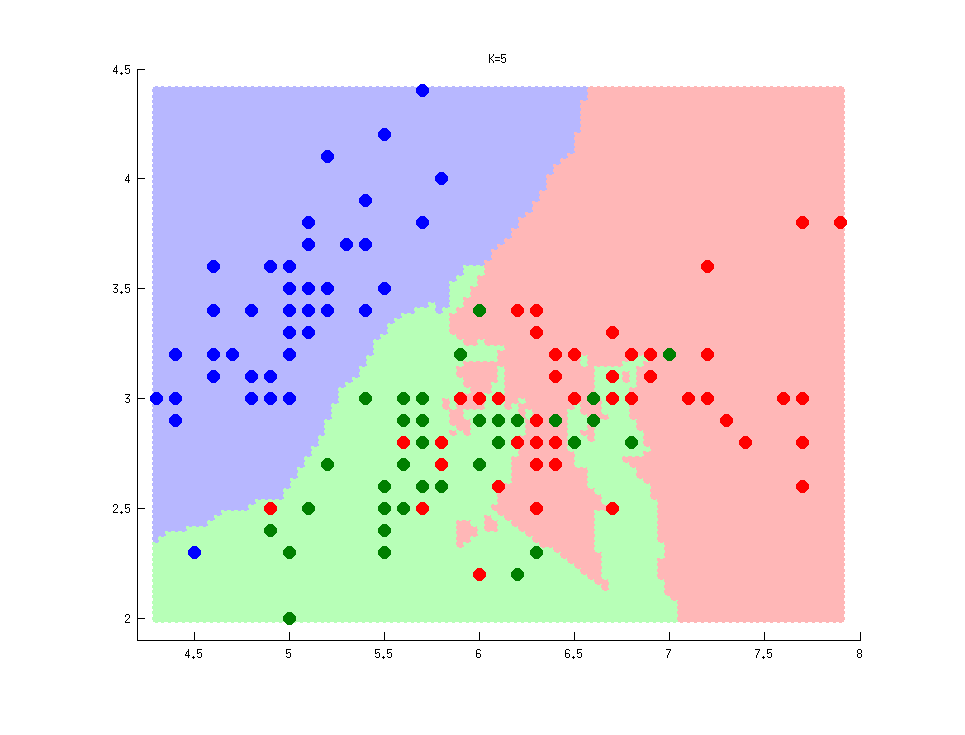
\includegraphics[width=70mm]{figuras/sepLVssepW/decRegK5.eps}
	  \\
	(a) k=1 & (b) k=5 \\[6pt] 
	 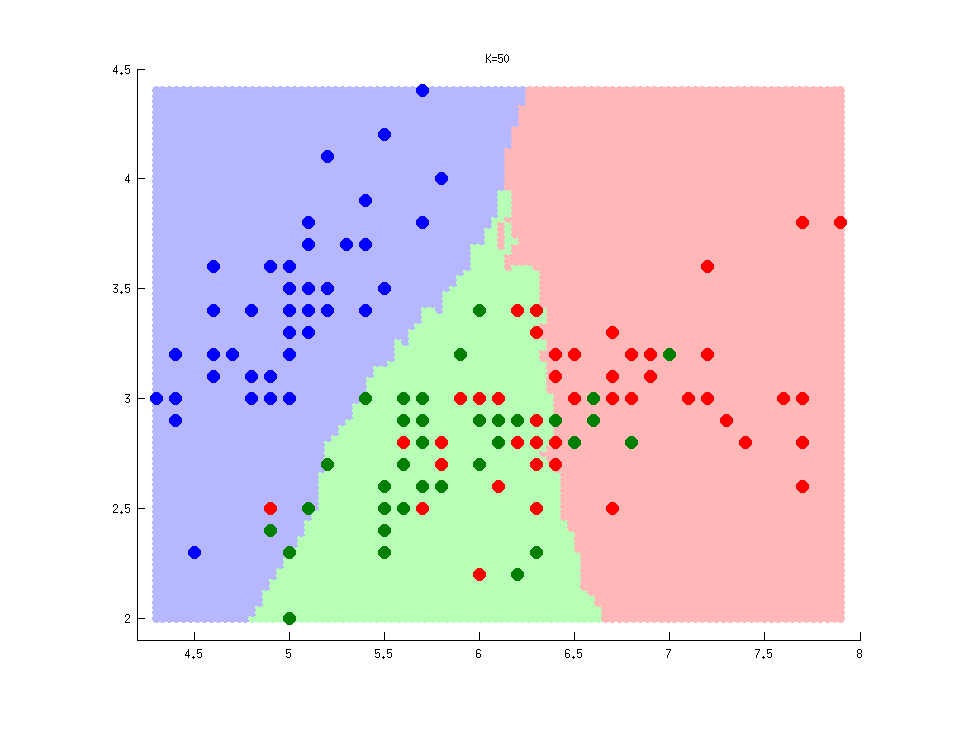
\includegraphics[width=70mm]{figuras/sepLVssepW/decRegK50.eps} &  
	 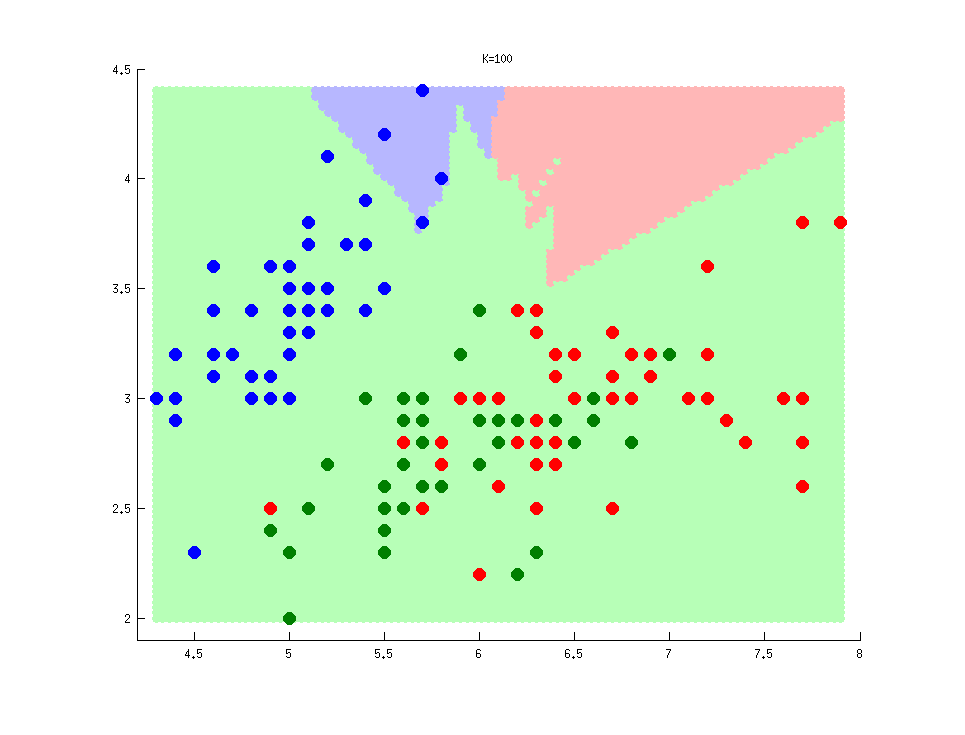
\includegraphics[width=70mm]{figuras/sepLVssepW/decRegK100.eps} \\
	(c) k=50 & (d) k=100 \\[6pt] 

	\end{tabular}
	\label{fig:decisionRegionSepL_SepW}
	\caption{Região de decisão utilizando comprimento e largura da sépala.}
\end{figure}


\section{Consulte o manual da classe \textsf{abntex2}}

Consulte o manual da classe \textsf{abntex2} \cite{abntex2classe} para uma
referência completa das macros e ambientes disponíveis.

% ---
% Finaliza a parte no bookmark do PDF, para que se inicie o bookmark na raiz
% ---
\bookmarksetup{startatroot}% 
% ---

% ---
% Conclusão
% ---
\section*{Considerações finais}
\addcontentsline{toc}{section}{Considerações finais}



% ----------------------------------------------------------
% ELEMENTOS PÓS-TEXTUAIS
% ----------------------------------------------------------
\postextual

% ----------------------------------------------------------
% Referências bibliográficas
% ----------------------------------------------------------
\bibliography{abntex2-modelo-references}
\bibliography{iris}

% ----------------------------------------------------------
% Glossário
% ------------------------------------ ----------------------
%
% Há diversas soluções prontas para glossário em LaTeX. 
% Consulte o manual do abnTeX2 para obter sugestões.
% 
%\glossary 

% ----------------------------------------------------------
% Apêndices
% ----------------------------------------------------------

% ---
% Inicia os apêndices
% ---
\begin{apendicesenv}

% ----------------------------------------------------------
\chapter{Nullam elementum urna vel imperdiet sodales elit ipsum pharetra ligula
ac pretium ante justo a nulla curabitur tristique arcu eu metus}
% ----------------------------------------------------------
\lipsum[55-57]

\end{apendicesenv}
% ---

% ----------------------------------------------------------
% Anexos
% ----------------------------------------------------------
\cftinserthook{toc}{AAA}
% ---
% Inicia os anexos
% ---
%\anexos
\begin{anexosenv}

% ---
\chapter{Cras non urna sed feugiat cum sociis natoque penatibus et magnis dis
parturient montes nascetur ridiculus mus}
% ---

\lipsum[31]

\end{anexosenv}


% ---
% Título e resumo em língua estrangeira
% ---

% \twocolumn[    		% INICIO DE ARTIGO EM DUAS COLUNAS

% titulo em inglês
\titulo{Canonical academic article model with \abnTeX}
\emptythanks
\maketitle

% resumo em português
\renewcommand{\resumoname}{Abstract}
\begin{resumoumacoluna}
 \begin{otherlanguage*}{english}
   According to ABNT NBR 6022:2003, an abstract in foreign language is a back
   matter mandatory element.

   \vspace{\onelineskip}
 
   \noindent
   \textbf{Key-words}: latex. abntex.
 \end{otherlanguage*}  
\end{resumoumacoluna}
 
% ]  				% FIM DE ARTIGO EM DUAS COLUNAS
% ---

\end{document}